\begin{center}
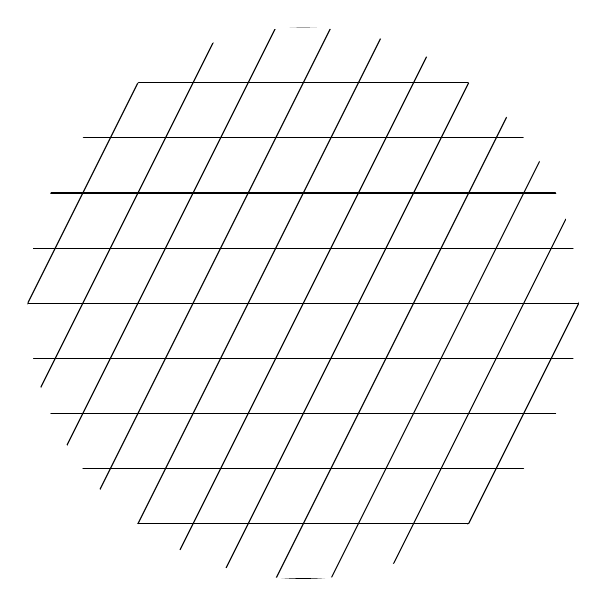
\begin{tikzpicture}[scale=0.7,every node/.style={scale=0.7}]
\placerpoint{A}{0}{0}{above left};
\placerpoint{B}{4}{0}{below right};
\placerpoint{C}{7.5}{5}{below right};
\placerpoint{D}{1}{2}{above left};
%\clip (-2,-0.1) rectangle (9,5.5);
\clip (4,2) circle (5);
%\foreach \y in {0, 1, ..., 10}{
	\foreach \x in {-10, ..., 10}{
		\begin{scope}[xshift=\x cm]
			\draw (-10,-20) -- (10,20);
		\end{scope}
		\begin{scope}[yshift=\x cm]
			\draw (-20,0) -- (20,0);
		\end{scope}
	}
%}
\end{tikzpicture}
\end{center}